\chapter{通信への応用}
    \section{2 経路交差フィルタ}
        \newcommand*{\xInI}{x_\text{i,I}}
        \newcommand*{\xInQ}{x_\text{i,Q}}
        \newcommand*{\xOutI}{x_\text{o,I}}
        \newcommand*{\xOutQ}{x_\text{o,Q}}
        \newcommand*{\hII}{h_\text{I,I}}
        \newcommand*{\hIQ}{h_\text{I,Q}}
        \newcommand*{\hQQ}{h_\text{Q,Q}}
        \newcommand*{\hQI}{h_\text{Q,I}}
        次のブロック図が示すフィルタを考える。
        これを「2 経路交差フィルタ」と呼ぶことにする。\footnote{筆者が勝手に付けた名前である。もし広く了解された名前を知っている読者が居たら,教えてほしい。}
        この構造は,典型的には直交変復調を用いる送信機に於いてアナログ回路の(余計な)周波数特性を補償するための DSP 機能として実装される。
        \begin{figure}[H]
            \centering
            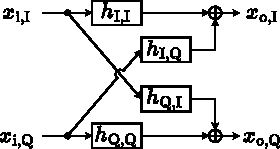
\includegraphics[keepaspectratio, scale=1]
            {\currfiledir/figs/two_path_cross_term_filter.pdf}
            \caption{2 経路交差フィルタのブロック図}
        \end{figure}
        ここに $\xInI,\;\xInQ,\;\xOutI,\;\xOutQ$ はそれぞれ入力の実数値信号,出力の実数値信号である。
        $\hII,\;\hIQ,\;\hQQ,\;\hQI$ は実数係数フィルタのインパルス応答である。
        \par
        以下の議論は,連続時間系,離散時間系の両方に適用でき,フィルタのインパルス応答は有限,無限どちらでもよい。
        そこで以下では連続時間系の無限インパルス応答フィルタを対象にする。
        入出力の関係式は次の通りである。
        \begin{equation}
            \label{equation:2 経路交差フィルタの入出力関係式}
            \begin{bmatrix}
                \xOutI \\
                \xOutQ
            \end{bmatrix} = \begin{bmatrix}
                \hII & \hIQ \\
                \hQI & \hQQ
            \end{bmatrix} *
            \begin{bmatrix}
                \xInI \\
                \xInQ
            \end{bmatrix}
        \end{equation}
        ここに,信号($\realNumbers\to\realNumbers$)を成分とする行列 $A, B$ 同士の畳み込み $A*B$ とは,通常の行列の積に於ける成分毎の積を畳み込みで置き換えたものと約束する。
    \subsection{複素係数フィルタと 2 経路交差フィルタの表現能力の違い}
        \ref{複素係数 feedforward フィルタの乗算回路の削減_導出} で扱った複素係数フィルタと 2 経路交差フィルタは似ているが,等価ではない。
        議論の解りやすさのために,前記複素係数フィルタを連続時間かつ無限インパルス応答に拡張する。入出力関係式は次式である。
        \begin{equation}
            \label{equation:複素係数フィルタの入出力関係式}
            \begin{bmatrix}
                \xOutReal \\
                \xOutImag
            \end{bmatrix} = \begin{bmatrix}
                \hReal & -\hImag \\
                \hImag & \hReal
            \end{bmatrix} *
            \begin{bmatrix}
                \xInReal \\
                \xInImag
            \end{bmatrix}
        \end{equation}
        \cref{equation:2 経路交差フィルタの入出力関係式} と \cref{equation:複素係数フィルタの入出力関係式} を比べて直ちに解るが,複素係数フィルタは 2 経路交差フィルタの特殊な場合である。
        前者は自由度が 4 ,後者は 2 である(係数列 1 個を 1 自由度と数える)。
    \section{直交復調}
        \newcommand*{\fc}{f_\text{c}}
        \subsection{直交復調は正の周波数側にある信号を取り出して中心周波数を 0 にする}
            キャリア周波数を $\fc$ ,入力である実時間信号を $x:\realNumbers\to\realNumbers$ とすると,直交復調器は $x(t)\parens*{\cos(2\pi \fc t) - i\sin(2\pi \fc t)}$ を LPF に通してベースバンドの外側の周波数成分を取り除く。
            その結果,ベースバンド信号として $X = \mathcal{F}(x)$ の正の周波数側の信号(複素数値信号)が得られる。
            \par
            そうなる理由を説明する。
            LPF に入力される前の信号の周波数表示された Fourier 変換は次式である。
            \[ \parens*{X*(\delta_{-\fc} + \delta_{\fc})/2}(f) - i\parens*{X*(\delta_{-\fc} - \delta_{\fc})/(2i)}(f) \]
            ここに $\delta_a\;(a\in\realNumbers)$ は Dirac のデルタ関数を時間軸方向に $-a$ だけシフトしたものである。
            計算を進めると次式を得る。
            \[ \frac{1}{2}\parens*{X(f-\fc)+X(f+\fc)} - \frac{1}{2}\parens*{X(f-\fc)-X(f+\fc)} = X(f+\fc) \]
            $x$ は実数値関数であるから $X$ は Hermite 対称である。
            つまり適当な $X_+:\realNumbers\to\complexNumbers$ が存在して,$X(f) = X_+(f) + \conj{X_+(-f)}$ である。
            さらに $X_+$ の台は $\fc$ を中心とするベースバンド帯域幅に制限されている。
            よって $X(f+\fc)$ を LPF に通した結果は $X_+(f)$ である。
    \section{Nyquist ISI 基準}
        これは大雑把に言うと Fourier 変換が存在する連続時間信号 $h:\realNumbers\to\complexNumbers$ が時刻 0 を除いて,ある周期 $\Ts>0$ (s は symbol の意味)の整数倍の時刻で 0 になるための必要十分条件である。
        限定された周波数帯域を使って通信する際に受信側で情報を正しく復元するために重要な性質であり,詳細は \cite{Nyquist_ISI_crit} にある。
        数式で表すと次である。
        \[
            h(n\Ts) = \begin{cases}
                1 & n=0 \\
                0 & n\in\integers\setminus\{0\}
            \end{cases}
            \iff \forall f\in\realNumbers,\;\frac{1}{\Ts}\sum_{n=-\infty}^\infty H(f-n/\Ts) = 1
        \]
        ここに $H$ は $h$ の Fourier 変換である。
        \cite{Nyquist_ISI_crit} には $\Rightarrow$ の証明のみがある。
        本書では $\Leftarrow$ を証明する。
        \begin{proof}
            \begin{align*}
                1 &= \frac{1}{\Ts}\sum_{n=-\infty}^\infty H(f-n/\Ts) = \frac{1}{\Ts}\sum_{n=-\infty}^\infty\integrate{-\infty}{\infty}{h(t)\exp\parens*{-i2\pi(f-n/\Ts)t}}{}{t} \\
                &= \frac{1}{\Ts}\integrate{-\infty}{\infty}{h(t)\exp(-i2\pi ft)\sum_{n=-\infty}^\infty\exp\parens*{i2\pi nt/\Ts}}{}{t} \tag{1}
            \end{align*}
            ここで次の関係式を使う(\ref{定数関数1のDTFT} の派生版)。
            \[ \sum_{n=-\infty}^\infty\exp\parens*{i2\pi nt/\Ts} = 2\pi\Ts\sum_{n=-\infty}^\infty\delta(2\pi t-2\pi\Ts n) = \Ts\sum_{n=-\infty}^\infty\delta(t-n\Ts) \]
            これを式 (1) に適用して次式を得る。
            \begin{align*}
                1 &= \integrate{-\infty}{\infty}{h(t)\exp\parens*{-i2\pi ft}\sum_{n=-\infty}^\infty\delta(t-n\Ts)}{}{t} = \sum_{n=-\infty}^\infty\integrate{-\infty}{\infty}{h(t)\exp\parens*{-i2\pi ft}\delta(t-n\Ts)}{}{t} \\
                &= \sum_{n=-\infty}^\infty h(n\Ts)\exp\parens*{-i2\pi fn\Ts}
            \end{align*}
            右辺は $f$ に関する周期 $1/\Ts$ の関数の Fourier 級数であり,$h(n\Ts)$ は Fourier 係数である。
            左辺が 1 であることから $h(0) = 1,\;h(n\Ts)\;(n\neq 0) = 0$ である(より丁寧に論じるなら,前記の式の両辺に $\exp(i2\pi fk\Ts)\;(k\in\integers)$ を掛けて区間 $[-1/(2\Ts),1/(2\Ts)]$ で積分する。その結果が $k$ にどう依存するかを調べる)。
        \end{proof}
    \section{帯域制限された信号が一定時間間隔で無限に配置されると定数になる}
        \begin{shadebox}
            $T>0$ とする。
            連続時間信号 $h:\realNumbers\to\complexNumbers$ の Fourier 変換 $H$ の台が有界であり,$H(f)=0\;(\abs{f}\geq 1/T)$ であるとき,次が成り立つ。
            \[ \sum_{n=-\infty}^\infty h(t-nT) = H(0)/T \]
        \end{shadebox}
        例えば位相変調による通信の目的で設計された回路に於いて,シンボル周期と同じ時間間隔で同じ大きさのパルスを Raised-Cosine フィルタに入力し続けると出力は一定の値になる。
        直感的には Raised-Cosine フィルタのインパルス応答が見えるように思えるが,そうはならない。
        \begin{proof}
            \begin{align*}
                \sum_{n=-\infty}^\infty h(t-nT) &= \sum_{n=-\infty}^\infty \mathcal{F}^{-1}(H)(t-nT) = \sum_{n=-\infty}^\infty\integrate{-\infty}{\infty}{H(f)\exp(i2\pi f(t-nT))}{}{f} \\
                &= \integrate{-\infty}{\infty}{H(f)\exp(i2\pi ft)\sum_{n=-\infty}^\infty\exp(-i2\pi fnT)}{}{f} \tag{1}
            \end{align*}
            ここで次の関係式を使う(\ref{定数関数1のDTFT} の派生版)。
            \begin{align*}
                \sum_{n=-\infty}^\infty\exp(-i2\pi fnT) &= \frac{2\pi}{T}\sum_{n=-\infty}^\infty\delta(-2\pi f - 2\pi n/T) = \frac{1}{T}\sum_{n=-\infty}^\infty\delta(-f - n/T) \\
                &= \frac{1}{T}\sum_{n=-\infty}^\infty\delta(f + n/T) = \frac{1}{T}\sum_{n=-\infty}^\infty\delta(f - n/T)
            \end{align*}
            これを式 (1) に適用して次式を得る。
            \begin{align*}
                \sum_{n=-\infty}^\infty h(t-nT) &= \frac{1}{T}\sum_{n=-\infty}^\infty\integrate{-\infty}{\infty}{H(f)\exp(i2\pi ft)\delta(f-n/T)}{}{f} \\
                &= \frac{1}{T}\sum_{n=-\infty}^\infty H(n/T)\exp(i2\pi nt/T) = H(0)/T
            \end{align*}
            最後の等号は $h$ の帯域制限の前提による。
        \end{proof}